\documentclass[main.tex]{subfiles}

\begin{document}
\section{程序运行测试}

\subsection{测试程序}
我使用老师提供的测试程序对系统进行测试,以下为添加注释后的测试程序源码:
\inputminted[linenos]{gas}{p1-test-commented.asm}

\clearpage

\subsection{调试辅助面板}
为了方便调试,我在主电路下方添加了一些调试辅助的功能,称作调试辅助面板。

主要是将主电路中的关键信号通过隧道引出,再与探针相连,并将它们按照指令类型、运算步骤分类,即形成了图中下半部分所示的调试辅助面板。

\begin{figure}[H]
\centering
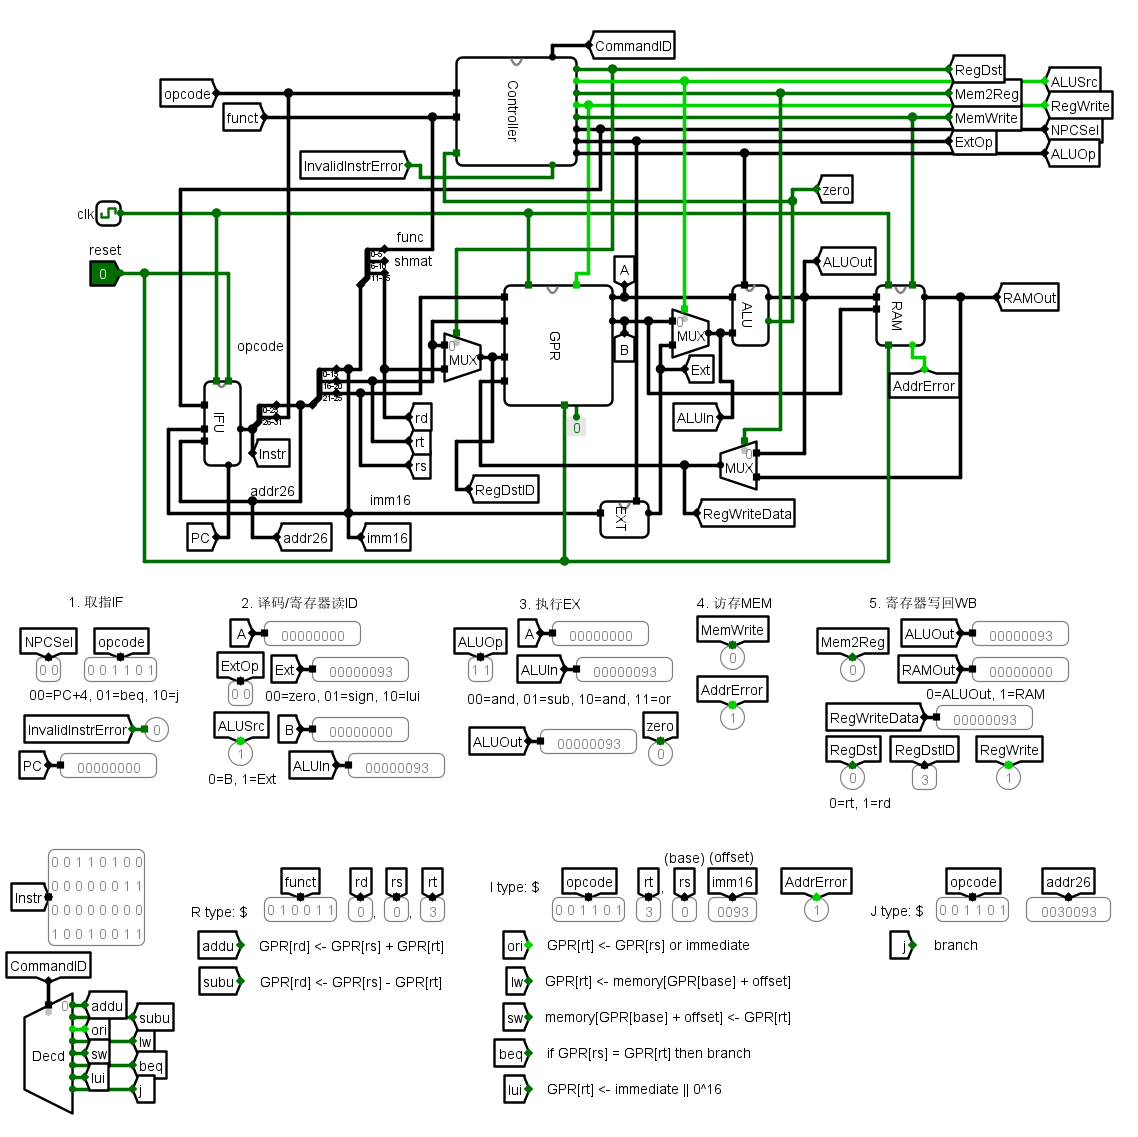
\includegraphics[width=\textwidth]{images/main-circuit.png}
\caption{main电路下方附加调试辅助面板}
\end{figure}

调试辅助面板可分为指令解析部分、各步骤状态部分。前者展示系统对指令的拆分、解析结果,后者展示各步骤的关键数据。

\subsection{测试报告格式}
按照要求,我会对每条指令进行一次测试,$beq$指令测试不同情况共两次。每次测试结果均以下述的测试报告格式写入此报告:

\paragraph{指令解析结果}
此部分会截取调试辅助面板指令解析部分,其中信息包含:指令类型判断、指令各操作数或立即数解析结果,并重新拼成类似汇编的形式便于检查。

\paragraph{各步骤运行中间参数}
此部分会截取调试辅助面板中各步骤的关键参数,用以判断每步运行过程均正确。

\paragraph{运行结果写入}
指令运行的结果一般分为三种:写回寄存器、写入主存、修改$PC$(对于跳转或条件跳转指令)。此部分会截取对应的写入结果(寄存器、主存、$PC$)。

\clearpage

\subsection{测试结果}
\newcommand{\instrtest}[5]{
\subsubsection{#2}
\paragraph{指令原文与预期效果}
测试ori指令,取测试程序中第#3行指令。

原文为:\mintinline{gas}{#4}。

效果为:#5

\paragraph{指令解析结果}
系统对指令解析后,重新拼接成类似汇编语言的指令,与原指令一致。

\begin{figure}[H]
\centering
\includegraphics[width=0.5\textwidth]{images/#1-instr.png}
\caption{#2测试-指令解析结果}
\end{figure}

\paragraph{各步骤运行中间参数}
各步骤运行中间参数均与预期一致。

\begin{figure}[H]
\centering
\includegraphics[width=\textwidth]{images/#1-steps.png}
\caption{#2测试-各步骤运行中间参数}
\end{figure}

\paragraph{运行结果写入}
运行结果写入效果与预期一致。

\begin{figure}[H]
\centering
\includegraphics[width=0.4\textwidth]{images/#1-result.png}
\caption{#2测试-运行结果写入}
\end{figure}

\clearpage
}

\instrtest{ori}{ori指令}{1}{ori $3,$0,0x93}{\$3写入0x0000\_0093}
\instrtest{addu}{addu指令}{3}{addu $8,$3,$6}{计算\$3(0x93)和\$6(0xae)的和,存入\$8(0x141)}
\instrtest{subu}{subu指令}{4}{subu $9,$3,$6}{计算\$3(0x93)和\$6(0xae)的差,存入\$9(-0x1b)}
\instrtest{sw}{sw指令}{6}{sw $9,16($0)}{将\$9(0x141)的值存入地址为0x10的内存}
\instrtest{lw}{lw指令}{7}{lw $10,16($0)}{将地址为0x10的内存数据(0x141)存入\$10}
\instrtest{beq-j}{beq指令(跳转)}{8}{beq $9,$10,l1}{比较\$9和\$10是否相等,\$9(0x141)==\$10(0x141),跳转到l1}
\instrtest{lui}{lui指令}{12}{lui $9,0x4567}{\$9写入0x4567\_0000}
\instrtest{j}{j指令}{13}{j l3}{跳转到l3}
\instrtest{beq-nj}{beq指令(不跳转)}{8}{beq $9,$10,l1}{比较\$9和\$10是否相等,\$9(0x45670000)$\neq $ \$10(0x141),执行下一条指令}

\subsubsection{寄存器\$0写入保护}
寄存器\$0的连线与其他寄存器不同,因此无法被写入。实际测试中,第5行指令会尝试向寄存器\$0中写入0x126,但运行到最终也没有写入,说明写入保护生效。
\begin{figure}[H]
\centering
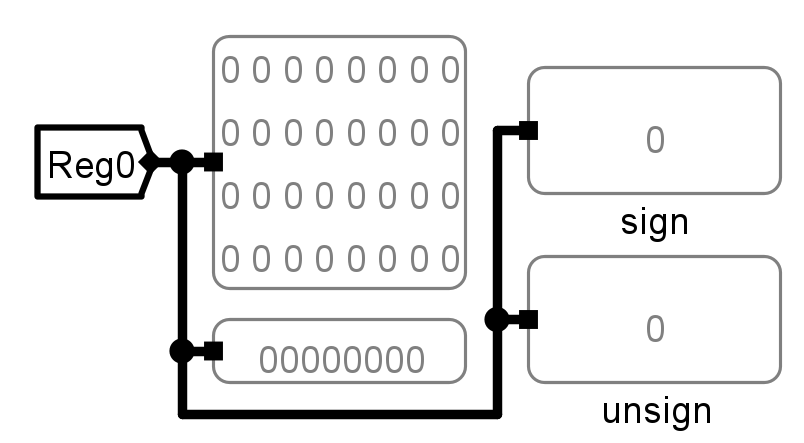
\includegraphics[width=0.4\textwidth]{images/reg0-final.png}
\caption{寄存器0最终状态}
\end{figure}


\end{document}
